\section{Experimental Setup and Measurement Process}
\label{sec:Experiment}
For the measurement of the refractive index of glass and air a Sagnac interferometer is used. Its setup and the measurement process used is explained in this section.
\subsection{Setup}
\label{sec:Setup}
The main feature of the Sagnac interferometer is the fact that both light beams travel the same path but in different directions. A schematic layout of a
Sagnac interferometer is depicted in \autoref{fig:Sagnac}.
\begin{figure}
    \centering
    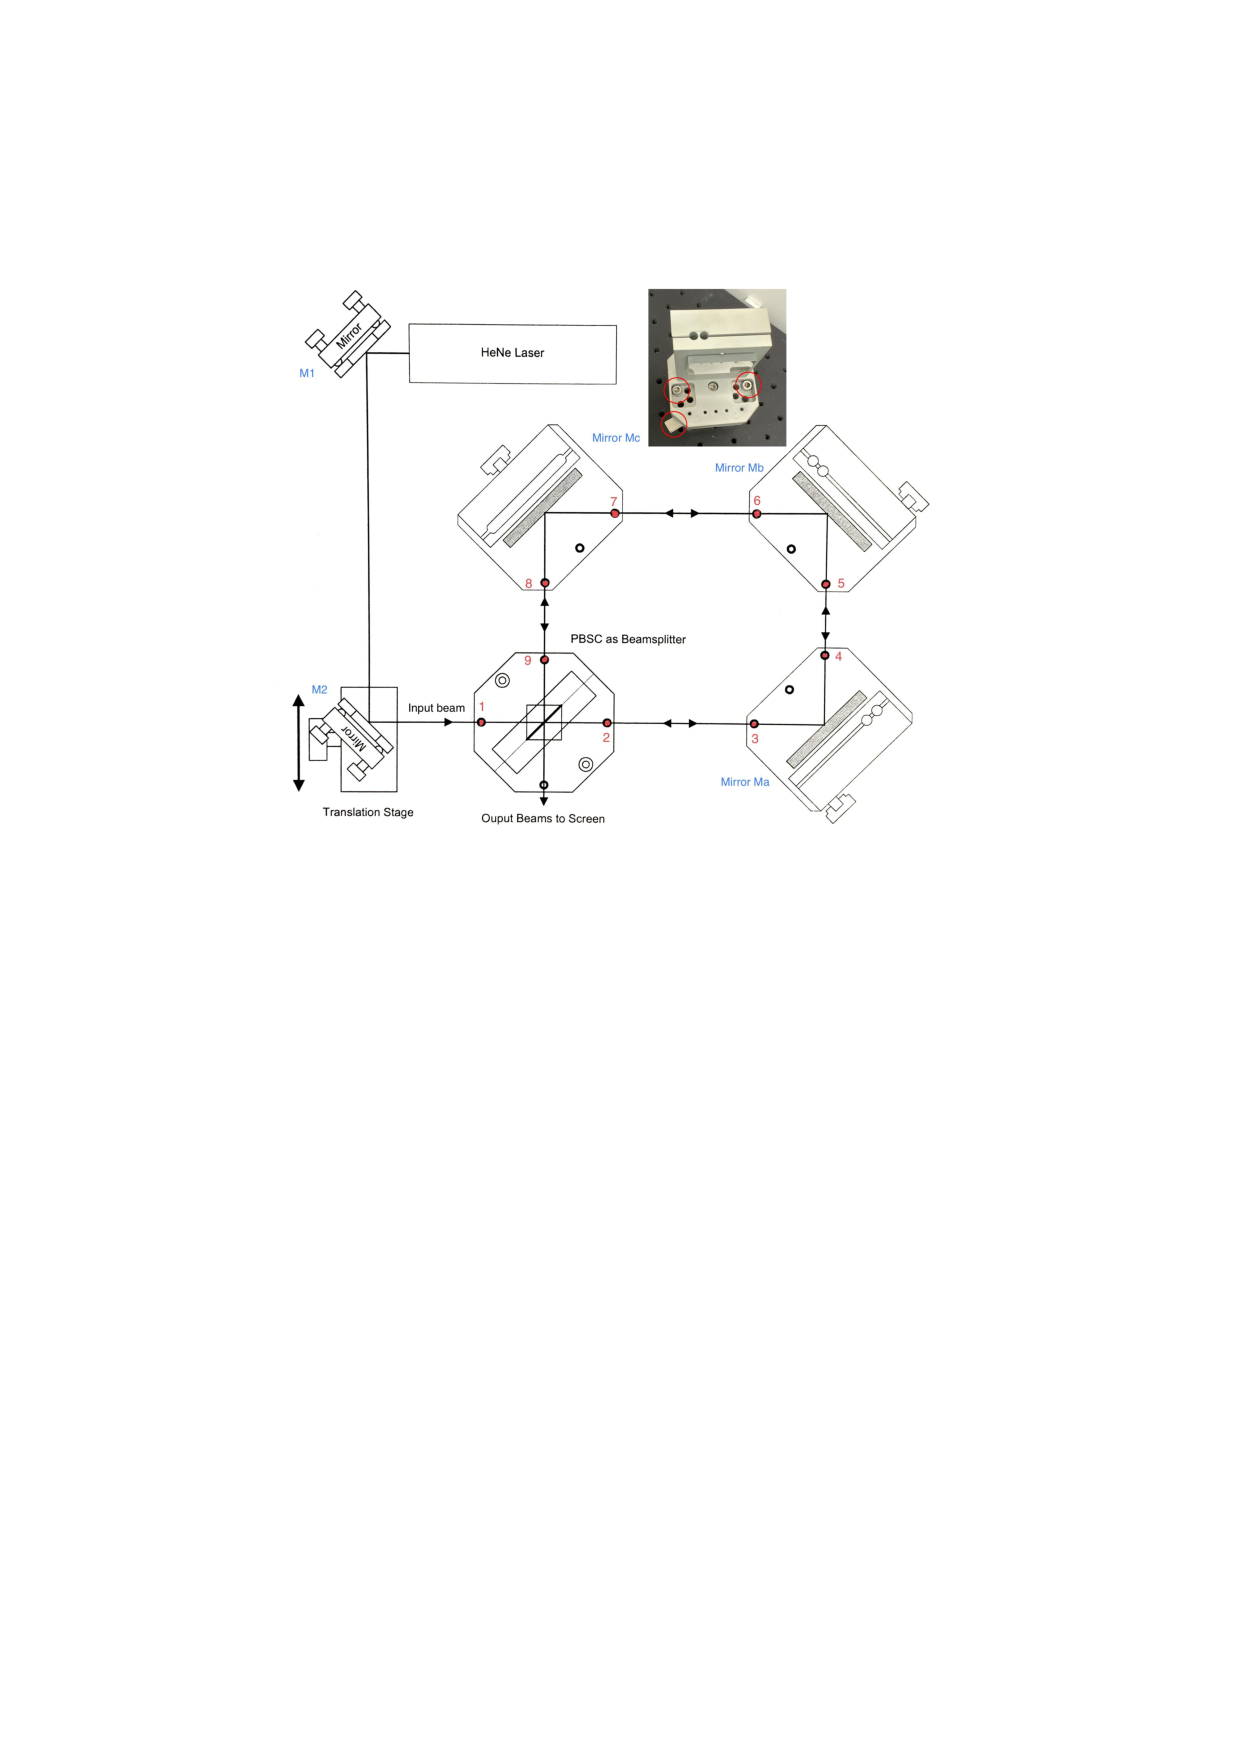
\includegraphics[height=10cm]{content/pics/setup.pdf}
    \caption{Layout of the Sagnac interferometer used in this experiment. The light beam is directed through the setup using several mirrors and is splitted into
    two beams at the PBSC \cite{v64}.}
    \label{fig:Sagnac}
\end{figure}
The input light beam is reflected by adjustable mirrors and passes through an adjustable polarization filter before it enters the PBSC. Here, it is split into its s- and p-polarized parts. The single beams are directed clockwise
and counterclockwise through the setup. Since the two light beams are differently polarized, a polarization filter is placed behind the output of the PBSC to filter out the 
parts of the beams that can interfer.
Before the intensity of the light beam is measured, it is split into the s- and p-polarized parts again using a PBSC. The intensity of the s- and p-polarized parts 
is determined using photodiods. The use of two photodiodes allows the implementation of a differential amplifier. The signal of the amplifier is connected to 
the read-out electronics that measure the number of intensity maxima.

\subsection{Measurement Process}
\label{sec:Measurement_process}
\subsubsection{Alignment of the Setup}
Before the actual measurements can start, the setup needs to be properly aligned. The light beams need to be spacially separated and adjusted so that they recombine
at the PBSC. It needs to be ensured that the beams are directed in one plane and do not diverge.

With the help of the adjustment screws at the mirrors, the setup is adjusted to achieve broad regions of destructive interference to maximize the contrast.

\subsubsection{Measurement of the Contrast}
\label{sec:Measure_contrast}
Once the interferometer is all aligned, the contrast is measured. Therefor, a piece of glass is placed into both beam paths. The optical instrument used here is tilted
by $\qty{+10}{\degree}$ for one beam and $\qty{-10}{\degree}$ for the other. The mount for this instrument can be rotated with a set screw.

The aim is to measure the contrast as a function of the polarization angle of the first polarization filter. A plexiglass hood covers the setup to suppress effects of
reflecion at air molecules. Finally, the intensity of the maxima and minima is measured at one photodiode using a voltmeter. The maxima and minima are set by turning the adjusting 
screw on the glass holder ever so slightly that the voltage maximizes or minimizes. This process is repeated three times for an angle range of $\qty{0}{\degree}≤\phi≤\qty{180}{\degree}$.

\subsubsection{Measurement of the Refractive Index of Glass}
\label{sec:Measure_n_Glass}
For the measurement of the refractive index of glass the read-out electronics that measure the number of maxima is used. The glass holder is rotated slowly for an
angle range of $\qty{0}{\degree}≤\theta≤\qty{8}{\degree}$ and the number of maxima is counted. This is performed ten times to reduce statistical uncertainties.

\subsubsection{Measurement of the Refractive Index of Air}
\label{sec:Measure_n_Air}
The refractive index of air is measured in a similar way. A cell that can be evacuated is placed in one of the light beams. By slowly increasing the cell pressure
the intensity maxima are again counted by the read-out electronics. The cell is evacuated and repressurized five times.